\section{Ejercicio 7}
En este experimento observaremos el error cuadrático medio para cada estimador en función de $n$, con $n$ siendo la cantidad de muestras de tamaño $15$. En el gráfico siguiente, podemos observar que errores cuadráticos medios de cada estimador convergen a valores no nulos. En particular, observando los datos adquiridos en el \textbf{ejercicio 4}, podemos observar que el error cuadrático medio de $\hat{\theta}_{mom}$ y $\hat{\theta}_{med}$ tienden a $0.022$ y $0.057$ respectivamente, que no coincidentalmente aproximan al valor de sus varianzas con $n \rightarrow \infty$.

\begin{figure}[H]
	\centering
	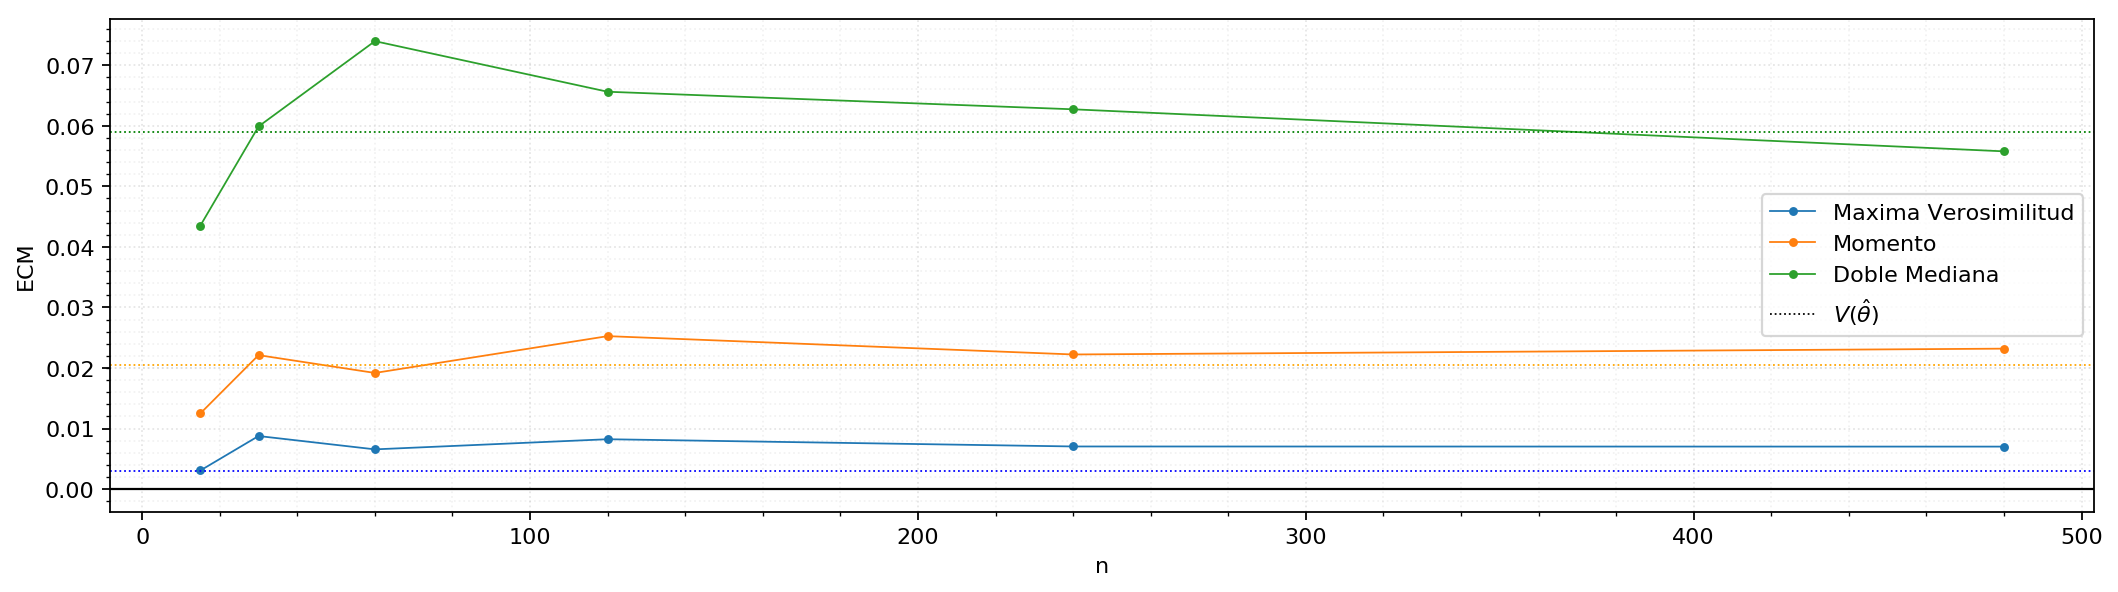
\includegraphics[width=1\textwidth]{imagenes/ecm-en-f-de-n.png}
	\caption{\footnotesize ECM de los estimadores en función de n. $a=0, b=1$}
	\label{fig:ej7-ecm-en-f-de-n}
\end{figure}